\section{边界判断：表达能力、真实深度、监督信号与部署位置}
\label{sec:limits-deployment}

本章结论是全文的冷水区：Loop Transformer 的研究价值真实存在，优势来自“用计算换有效深度，用共享参数换紧凑模型”；它尚未被证明可以作为标准 Transformer 或思维链（Chain-of-Thought, CoT）的通用替代方案。它能否成为实用路线，取决于表达能力、真实深度、监督信号、KV cache 和部署约束能否同时过关。

\begin{importantbox}{本章主张}
Loop Transformer 适合被理解为一种带强归纳偏置的递归计算方案。它把模型推向“反复更新同一份隐藏表示”的路线；标准 Transformer 的深层堆栈则给每一层独立参数和独立变换空间。二者的系统价值要按任务、内存、延迟和训练信号共同判断。
\end{importantbox}

\subsection{表达能力：共享权重是一种约束}

表达能力（expressiveness）指模型函数族能表示多复杂的输入输出关系。视频在 00:14:48--00:15:17 提醒读者：拥有独立层的更深或更宽模型通常有更大的自由度；如果内存和参数预算宽松，标准 Transformer 可以通过增加层数、宽度和参数量获得更低损失，并避开递归 KV 管理的复杂性。

用公式先表达结构差异。独立深层堆栈把多个不同变换串起来；递归深度把同一个共享变换反复应用。这个公式只说明架构约束，不能直接推出哪个模型在所有任务上更强。

$$
h_L = F_L\circ F_{L-1}\circ \cdots \circ F_1(x),\qquad
h_R = \underbrace{F_\theta\circ F_\theta\circ \cdots \circ F_\theta}_{R\ \mathrm{steps}}(x)
$$

\begin{itemize}
  \item \(x\)：输入 token 或输入隐藏表示。
  \item \(h_L\)：经过 \(L\) 个独立层后的表示。
  \item \(F_1,\ldots,F_L\)：每层各自拥有参数的 Transformer 变换。
  \item \(h_R\)：经过 \(R\) 次递归后的表示。
  \item \(F_\theta\)：参数 \(\theta\) 共享的循环模块。
  \item \(\circ\)：函数复合，表示前一个变换的输出进入下一个变换。
\end{itemize}

\begin{figure}[htbp]
  \centering
  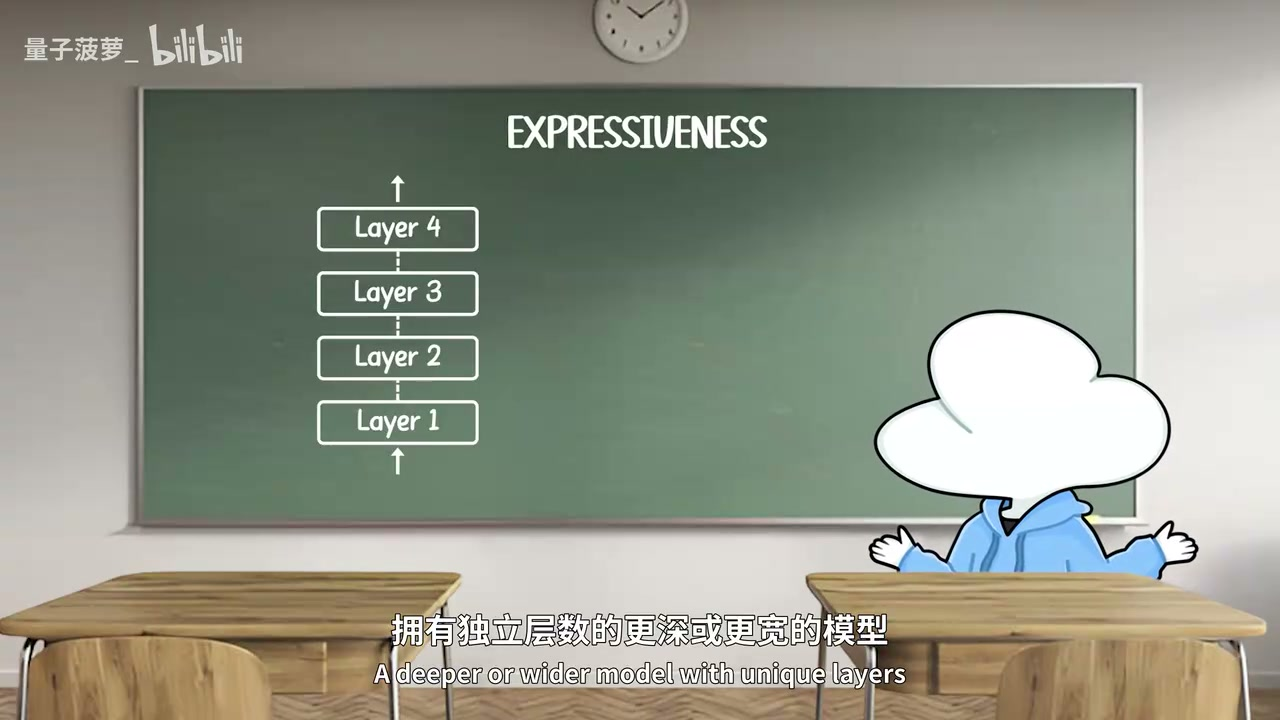
\includegraphics[width=0.82\linewidth,height=0.36\textheight,keepaspectratio]{figures/fig_15_expressiveness_comparison.jpg}
  \caption{表达能力边界：独立深层或更宽模型拥有更大的参数自由度，共享递归块是一种更紧凑的受约束选择。\protect\footnotemark}
  \label{fig:expressiveness-comparison}
\end{figure}
\footnotetext{视频画面时间区间：00:14:48--00:15:17。}

这里有一个容易漏掉的背景：扩展定律（scaling laws）的历史经验更偏向增加参数量和数据量。重复利用计算想要成为主路线，需要证明它在同等系统预算下带来更高质量、更低成本或更好的可部署性。

\subsection{真实深度与递归深度}

真实深度（real depth）意味着每一层都可以学习自己的变换；递归深度（recurrent depth）意味着同一函数在不同状态上重复执行。前者给模型显式的分层归纳偏置，后者依赖隐藏状态的演化让同一共享模块在早期、中期、后期表现出不同功能。

上一章之前的机制分析给了积极信号：共享块在不同递归阶段可能承担粗略表示、关系整合、答案收敛等角色。边界也同样明确：这种阶段化行为需要模型自己学出来；独立深层堆栈把“每一步可以不同”直接写进参数结构里。

\begin{figure}[htbp]
  \centering
  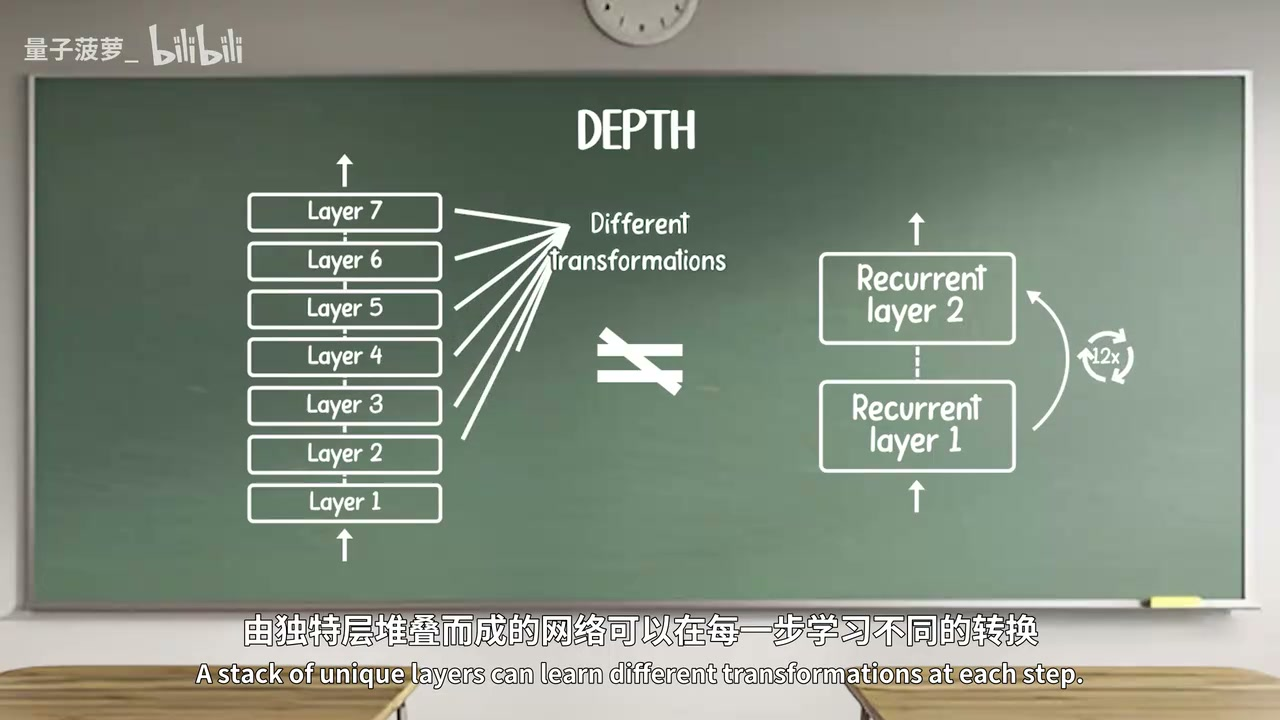
\includegraphics[width=0.82\linewidth,height=0.36\textheight,keepaspectratio]{figures/fig_16_depth_comparison.jpg}
  \caption{真实深度与递归深度的差异：独立层提供不同变换，循环层复用同一函数并依赖状态演化产生阶段差异。\protect\footnotemark}
  \label{fig:depth-comparison}
\end{figure}
\footnotetext{视频画面时间区间：00:15:31--00:16:10。}

\begin{warningbox}{深度误读}
把“循环次数更多”直接读成“模型等价于更深的 Transformer”会误导判断。递归深度增加了计算步数，也增加了同一函数反复作用的机会；真实深度增加的是可学习变换的种类和参数自由度。
\end{warningbox}

\subsection{推理收益的证据边界}

视频对多跳推理和深度外推保持了谨慎态度。受控基准中的多跳结果很有价值，因为它们说明递归深度可能形成可复用的计算过程；这些结果距离大规模真实任务还有距离。真实任务包含长上下文噪声、开放域知识、工具调用、格式约束、多轮交互和分布漂移，循环深度在这些条件下能否稳定贡献收益，需要更多实验。

这也是“房间里的大问题”：如果计算和内存允许，直接加深或加宽标准 Transformer 可能更简单；如果参数预算很紧，Loop Transformer 才更容易显出独特价值。研究判断要追问的是边际收益：多花一次递归步，和多加一层独立层、多生成若干 CoT token、增大批量或优化 KV cache 相比，哪个更划算。

\subsection{CoT 的监督信号优势}

CoT 的工程价值除了推理时多写 token，还在于它留下了显式文本轨迹。这些轨迹可以被人工筛选，可以用于监督学习，可以作为强化学习的过程信号，也可以被学生模型模仿。换句话说，CoT 把“思考过程”变成可存储、可审查、可训练的数据。

Loop Transformer 的隐藏状态递归更紧凑，也更难监督。中间计算藏在连续向量里，没有自然语言标签告诉模型第一步、第二步、第三步应如何组织。训练只能更多依赖最终目标，或者依赖额外的探针、辅助损失、蒸馏教师和轨迹约束。这些方案有研究空间，也会增加训练设计难度。

\begin{figure}[htbp]
  \centering
  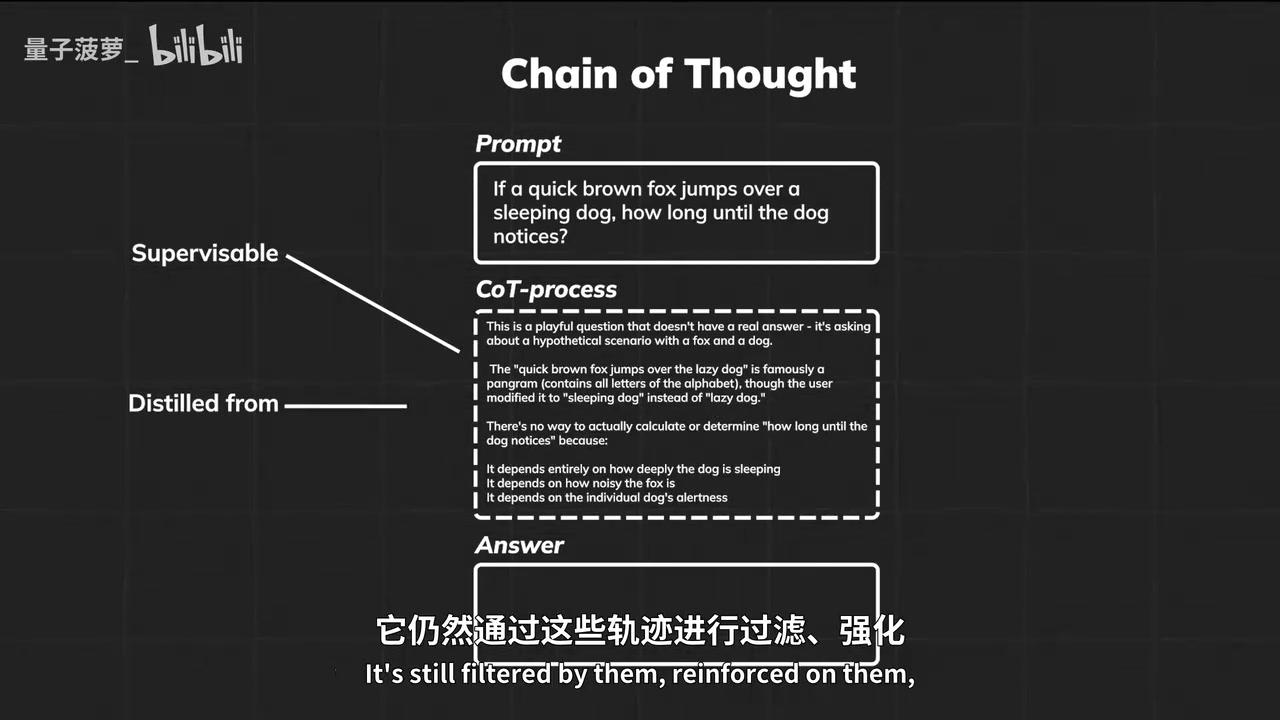
\includegraphics[width=0.82\linewidth,height=0.36\textheight,keepaspectratio]{figures/fig_17_cot_vs_looped_model.jpg}
  \caption{CoT 的显式轨迹优势：文本中间步骤便于监督、筛选、强化和蒸馏；隐藏状态递归缺少天然中间标签。\protect\footnotemark}
  \label{fig:cot-vs-looped-model}
\end{figure}
\footnotetext{视频画面时间区间：00:16:34--00:17:23。}

\begin{knowledgebox}{监督信号类比}
可以把 CoT 轨迹理解为学生写在草稿纸上的解题步骤。教师能批改每一步，挑出好草稿，训练另一个学生模仿。隐藏状态递归更像学生在脑内默算，答案也许正确，教师很难知道中间哪一步值得奖励或修正。
\end{knowledgebox}

\subsection{可能的部署位置}

视频给出的潜在落点集中在资源受限或同参数竞争场景：合成数据生成（synthetic data generation）、蒸馏（distillation）、边缘部署（edge deployment）、移动设备小模型，以及 CoT 成本过高或同参数模型能力不足的场景。这里的关键词是“约束”。当参数容量是主要瓶颈，递归计算能把有限参数重复使用；当服务瓶颈是延迟和吞吐，重复模块的序列化成本会变得刺眼。

\begin{figure}[htbp]
  \centering
  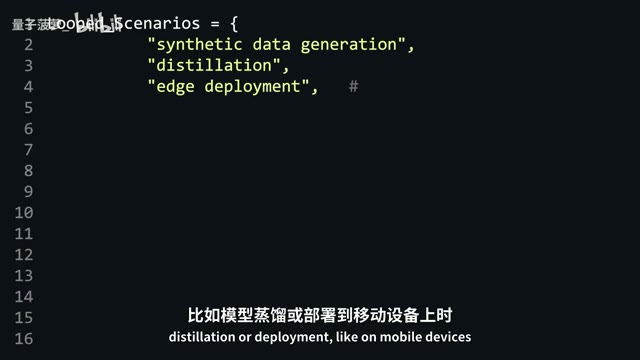
\includegraphics[width=0.72\linewidth,height=0.30\textheight,keepaspectratio]{figures/fig_18_application_scenarios.jpg}
  \caption{潜在应用场景：合成数据生成、蒸馏和边缘部署更容易体现共享参数与递归计算的价值。\protect\footnotemark}
  \label{fig:application-scenarios}
\end{figure}
\footnotetext{视频画面时间区间：00:17:23--00:17:40。}

实践者应把 Loop Transformer 放进系统指标里评估：同等参数量下质量是否提升，同等延迟下吞吐是否下降，长上下文 KV cache 是否可控，路由器是否稳定，训练数据中是否存在足够的过程信号。少看单点指标，多看质量、成本和部署约束的共同边界。

\subsection{本章小结}

本章形成三点判断：

\begin{itemize}
  \item Loop Transformer 的优势来自用计算换有效深度，用共享参数换紧凑模型；它的代价是表达能力约束、递归状态管理和更难监督的内部过程。
  \item 它的研究价值取决于稳定性、自适应路由、KV cache 和训练监督能否一起成立；只解决其中一项，仍不足以支撑大规模默认替代路径。
  \item 它近期更像特定约束下的工程与研究选项，尤其适合小模型、边缘部署、蒸馏和同参数量竞争；在大规模 LLM 服务中，标准 Transformer 与 CoT 仍拥有强大的训练、扩展和部署惯性。
\end{itemize}
